\documentclass[11pt, letterpaper]{article}

% Essential Packages
\usepackage{amsmath, amssymb, amsthm} % Math symbols and environments
\usepackage{enumitem}
\usepackage[margin=1in]{geometry}       % Page margins
\usepackage{fancyhdr}                   % Custom headers and footers
\usepackage{listings}                   % For including code snippets
\usepackage{xcolor}                     % For colored text/code highlighting
\usepackage{graphicx}                   % For including images

% Header and Footer Setup
\pagestyle{fancy}
\fancyhead[L]{ANANDAN IYER\\Roll No. : 240117\\Mechanical Engg.}
\fancyhead[C]{CGS698C\\Bayesian Models and Data Analysis\\Assignment \#2}
\fancyhead[R]{\today}
\setlength{\headheight}{26pt}

% Code Listing Configuration
\definecolor{codegray}{rgb}{0.5,0.5,0.5}
\definecolor{backcolour}{rgb}{0.95,0.95,0.92}

\lstdefinestyle{mystyle}{
    backgroundcolor=\color{backcolour},
    basicstyle=\ttfamily\footnotesize,
    breakatwhitespace=false,
    breaklines=true,
    captionpos=b,
    keepspaces=true,
    numbersep=5pt,
    showspaces=false,
    showstringspaces=false,
    showtabs=false,
    tabsize=2
}
\lstset{style=mystyle}

% Custom Environment for Problems
\newenvironment{problem}[2][Problem]
    {\section*{#1 #2}}
    {}

\begin{document}

%--- Content Starts Here ---%

\begin{problem}{1: Continuous random variables}
\end{problem}

\textbf{Solution :}

\textbf{1.1} The sample space of the experiment for analyzing the accuracy of the shooter in terms of the distance from the target : \newline 
$\Omega = \{(m_1,m_2,m_3,m_4,m_5) \mid m_i \in \mathbb{R}, m_i \ge 0\}$. \newline 
Given, a random variable $X$ as a function of $\omega$ which maps to a discrete space $\Omega_x$ where the margin of failure and success is determined whether the target is missed by 5 cm or not respectively. \newline \newline
(a) $X(\omega) = \sum_{i=1}^{5} f(m_i \le 5)$, where $f$ indicates the margin for success s.t. $m_i \le 5cm$ which matches the failure condition. \newline\
(b) The probability function for the random variable $X(\omega)$ can be given by the binomial distribution $P$. $P(X=k) = \binom{5}{k}p^k(1-p)^{5-k}$ for $k \in \{0, \dots, 5\}$ where $k$ represents a "failure" event defined by the random variable $X$. \newline

\textbf{1.2} The probability density function of the normal distribution is given by 
$f(x) = \frac{1}{\sigma\sqrt{2\pi}} e^-{\frac{(x-\mu)^2}{2\sigma^2}}$\newline\newline
(a) Given, $x = 0, \mu = 1, \sigma = 1$\newline
$\implies f(0) = \frac{1}{1.\sqrt{2\pi}}e^-{\frac{(0-1)^2}{2.1^2}}$ \newline
$\implies f(0) = \frac{1}{\sqrt{2\pi}}e^-\frac{1}{2}$ \newline
$\implies f(0) \approx 0.242$ \newline
(b) Given, $x = 1, \mu = 0, \sigma = 1$\newline
$\implies f(1) = \frac{1}{1.\sqrt{2\pi}}e^-{\frac{(1-0)^2}{2.1^2}}$ \newline
$\implies f(1) = \frac{1}{\sqrt{2\pi}}e^-\frac{1}{2}$ \newline
$\implies f(1) \approx 0.242$ \newline
(c) $P(x_2 \le X \le x_3) = P(x_1 \le X \le x_3) - P(x_1 \le X \le x_2) = 0.45 - 0.3 = 0.15$. \newline

\textbf{1.3} The continuous random variable $X$ has the probability density function given by $f(x) = \frac{(\alpha + \beta - 1)!}{(\alpha - 1)!(\beta - 1)!}x^{\alpha - 1}(1-x)^{\beta - 1}$ \newline \newline 
The mode is found by solving $\frac{d}{dx}f(x) = 0$ \newline
$\implies \frac{d}{dx}\frac{(\alpha + \beta - 1)!}{(\alpha - 1)!(\beta - 1)!}x^{\alpha - 1}(1-x)^{\beta - 1} = 0 \implies K\frac{d}{dx}x^{\alpha - 1}(1-x)^{\beta - 1} = 0 \newline \implies (\alpha - 1)x^{\alpha - 2}(1-x)^{\beta - 1} - (\beta - 1)x^{\alpha - 1}(1-x)^{\beta - 2} = 0$\newline $\implies x^{\alpha - 2}(1-x)^{\beta -2}((\alpha - 1)(1-x) - (\beta - 1)x) = 0$ \newline Disregarding the trivial solution, \newline $\implies x(\beta - 1 + \alpha -1) = \alpha -1 \implies x = \frac{\alpha -1}{\alpha + \beta - 2}$ \newline
$\therefore$ The mode of the random variable $X$ = $\frac{\alpha -1}{\alpha + \beta - 2}$
\newline 

\textbf{1.4} Standard Normal of a Probability Density Function $f(x) = \frac{1}{\sqrt{2\pi}}e^{-x^2/2}$: \newline
\newline
(a) Comparing the given $f(x)$ with a Standard Probability Density Function $g(x) = \frac{1}{\sigma\sqrt{2\pi}} e^{-\frac{(x-\mu)^2}{2\sigma^2}}$, \newline The mean $\mu = 0$ \newline The variance $\sigma^2 = 1$ \newline
(b) Density at $x = 0 \implies$ Density at $f(0) = \frac{1}{\sqrt{2\pi}}e^\frac{-0^2}{2} \implies f(0) = \frac{1}{\sqrt{2\pi}} \approx 0.3989$ \newline
(c) The probability density graph is symmetric about $x = 0 \implies P(X < 0) = 0.5$ \newline
(d) For any continuous random variable, the probability of obtaining an exact point value is always 0 $\therefore P(X = 0) = 0 \square$
\newline
\vspace{3pt}
%--------------------------------------------------%

\begin{problem}{2: The distribution of distances between related words in natural languages}
\end{problem}

\textbf{Solution:} \newline
The probability mass function that we're following: $f(k, \lambda) = \frac{\lambda^{k}e^{-\lambda}}{k!}$ where $k$ is the linear distance between the word pairs. \newline
English: $f(k) = \frac{\lambda_{1}^{k}e^{-\lambda_{1}}}{k!}$ \newline
German: $f(k) = \frac{\lambda_{2}^{k}e^{-\lambda_{2}}}{k!}$ \newline
Czech: $f(k) = \frac{\lambda_{3}^{k}e^{-\lambda_{3}}}{k!}$ \newline

\textbf{2.1} at distance 0, $k=0 \therefore f(0) = \frac{\lambda^{0}e^{-\lambda}}{0!} = e^{-\lambda}$ \newline
Note, $\lambda_{3} < \lambda_{1} < \lambda_{2} \therefore$ The language with the smallest $\lambda$ wins. Hence, Czech ($\lambda_{3}$) has the highest word pairs with linear distance = 0. \newline

\textbf{2.2} Number of word pairs for $k=1$, $f(1, \lambda) = \lambda e^{-\lambda}$. \newline
The no. of related word pairs with linear distance = 1, given the total number of words in English, German and Czech corpora is $10^5, 10^7$ and $10^9$: \newline
For English, $f(1, \lambda) = 10^{5} \times 0.7 \times e^{-0.7} \simeq 34,760$ \newline
For German, $f(1, \lambda) = 10^{7} \times 0.8 \times e^{-0.8} \simeq 3,595,000$ \newline
For Czech, $f(1, \lambda) = 10^{8} \times 0.6 \times e^{-0.6} \simeq 32,930,000$ \newline

\textbf{2.3} For a random structure corpus, $f(k) = \frac{2^{k}e^{-2}}{k!}$ \newline
The structures have relatively longer distances between related nodes when compared to natural language structures which peaks at $k=0$ (when $\lambda \le 1$). However, the random structure corpus represents a Poisson distribution with $\lambda = 2$.
\newline
\vspace{3pt}
%--------------------------------------------------%

\newpage \begin{problem}{3: The likelihood function}
\end{problem}

\textbf{Solution:}

\textbf{3.1} A researcher proposes a hypothesis that the string recognition times are generated by the probability density function $f(x, \mu): X \sim f(x, \mu)$ such that, $f(x, \mu) = \frac{1}{x\sqrt{2\pi}}e^{-\frac{(\log x - \mu)^2}{2}}$
\newline
(a)
\begin{center}
    
\includegraphics[width=0.8\textwidth]{Figure_1.png}
\end{center}
\newline
(b)
\begin{center}
    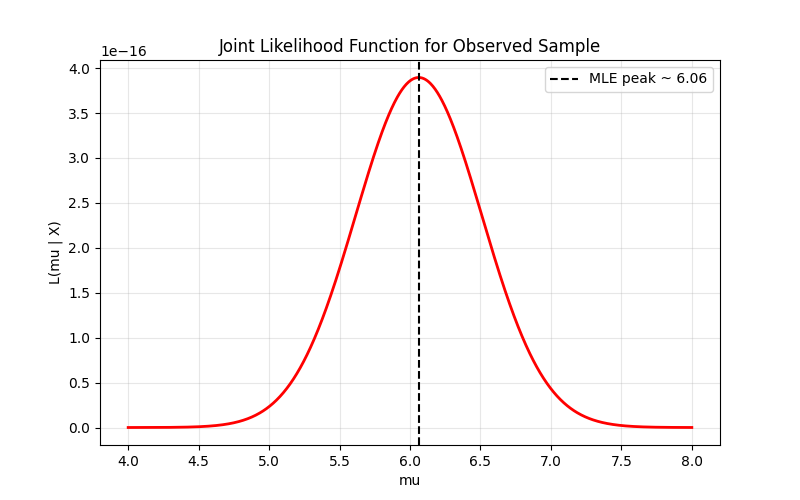
\includegraphics[width=0.8\textwidth]{Figure_2.png}
\end{center}
\newline
(c) MLE for the distribution is maximized when the value of $\mu$ is given by,
$$\hat{\mu} = \frac{\sum \log(x_{i})}{n} \simeq 6.06$$

\vspace{3pt}
%--------------------------------------------------%

\begin{problem}{4: Distributions in R}
\end{problem}

\textbf{Solution:}

\textbf{4.1} 
\newline
(a) The probability of obtaining a value of 700 or less = \textbf{0.9772}
\newline
(b) The probability of obtaining a value of 900 or more = \textbf{0.0000}
\newline
(c) The probability of obtaining a value between 200 and 800 = \textbf{0.9973}
\newline

\textbf{4.2} The
probability density of obtaining a value of 550 from this distribution = \textbf{0.002318}
\newline

\textbf{4.3} From the vector \textit{$x$sim}, \newline
Mean = \textbf{299.57}
\newline Standard Deviation = \textbf{200.68}
\newline Minimum = \textbf{-484.48}
\newline Maximum = \textbf{1085.25}
\newline 

\appendix
\section*{References}
\addcontentsline{toc}{section}{References}

The following Python scripts were used to generate the likelihood function plots and perform the statistical calculations for this assignment.

\begin{lstlisting}[language=Python, caption={Python script for Part 3.1 Likelihood Plots}]
import numpy as np
import matplotlib.pyplot as plt

x_obs = np.array([303.25, 443, 220, 560, 880])
m_vals = np.linspace(4, 8, 1000)

plt.figure(figsize=(8, 5))
y_a = (1/(220 * np.sqrt(2 * np.pi))) * np.exp(-((np.log(220) - m_vals)**2) / 2)
plt.plot(m_vals, y_a, color='blue', linewidth=2)
plt.title('Likelihood Function for x = 220')
plt.xlabel('mu')
plt.ylabel('L(mu | x=220)')
plt.grid(True, alpha=0.3)
plt.show()

plt.figure(figsize=(8, 5))
def joint_lik(m, xs):
    n = len(xs)
    prod_x = np.prod(xs)
    term1 = 1/(prod_x*(np.sqrt(2 * np.pi)**n))
    term2 = np.exp(-np.sum((np.log(xs) - m)**2) / 2)
    return term1*term2

y_b = [joint_lik(m, x_obs) for m in m_vals]
mle_val = np.mean(np.log(x_obs))

plt.plot(m_vals, y_b, color='red', linewidth=2)
plt.axvline(mle_val, color='black', linestyle='--', label=f'MLE peak ~ {mle_val:.2f}')
plt.title('Joint Likelihood Function for Observed Sample')
plt.xlabel('mu')
plt.ylabel('L(mu | X)')
plt.legend()
plt.grid(True, alpha=0.3)
plt.show()
\end{lstlisting}

\begin{lstlisting}[language=Python, caption={Python script for Part 4 Statistical Calculations}]
import numpy as np
import matplotlib.pyplot as plt
from scipy.stats import norm, binom, poisson

p41a = norm.cdf(700, 500, 100)
p41b = 1 - norm.cdf(900, 500, 100)
p41c = norm.cdf(800, 500, 100) - norm.cdf(200, 500, 100)

dens_42 = norm.pdf(550, 650, 125)

np.random.seed(42) 
xsim = np.random.normal(300, 200, 10000)
sim_mean = np.mean(xsim)
sim_sd = np.std(xsim)
sim_min = np.min(xsim)
sim_max = np.max(xsim)

print(f"4.1(a): {p41a:.4f}, (b): {p41b:.4f}, (c): {p41c:.4f}")
print(f"4.2 Density at 550: {dens_42:.6f}")
print(f"4.3 Sim Mean: {sim_mean:.2f}, SD: {sim_sd:.2f}, Min: {sim_min:.2f}, Max: {sim_max:.2f}")
\end{lstlisting}

\vspace{3pt}
\end{document}